\chapter{Réaliser des graphiques}
\backgroundimage{img/ch3}
\thispagestyle{chapterpage}

\newpage

\section{Le package tikz-pgf}

Il existe de nombreux paquets qui permettent de faire des graphiques. L'un des paquets les plus riches est \verb|pgf| (\url{https://www.ctan.org/pkg/pgf}) . Son manuel d'utilisation fait 1161 pages ! On peut trouver des exemples de ce qu'on peut faire sur le site \href{http://www.texample.net/tikz/examples/area/mathematics/}{texample.net}.

Pour les besoins d'un manuel de maths, voici les graphiques que j'utilise de plus souvent:


\section{Graphiques de fonctions}

\subsection*{Fonction définie par une expression}



\begin{tcblisting}{colback=red!5!white,colframe=red!75!black,listing above text}
\begin{tikzpicture}[scale=1,general]
    \window{-6}{8}{-30}{50} 
    \begin{windowsratio}
    \draw[xstep=1,ystep=10,grid] (\Xmin,\Ymin) grid (\Xmax,\Ymax);
    \axeH;\axeV;\tickX;\tickY[10];
    \node[below left] at (0,0) {0 };
    \clip (\Xmin,\Ymin) rectangle (\Xmax,\Ymax);
    \def \f{-\x^3+5*(\x)^2+10*\x-15};
    \draw[samples=100,domain=-6:8,courbe]
       plot(\x,{\f});     
    \end{windowsratio}
\end{tikzpicture}
\end{tcblisting}







L'argument \verb|general| permet d'avoir le même style pour toutes les figures (par exemple la couleur et l'épaisseur du quadrillage).

Les commandes \verb|\window|, \verb|\axeH|, \verb|\axeV|, \verb|\tickX| et \verb|\tickY| ainsi que l'environnement \verb|windowsratio| sont propres au package \verb|eshmathbook|.

Les autres commandes appartiennent au package \verb|pgf|. 


\subsection*{Courbe qui passe par des points donnés}


\begin{tcblisting}{colback=red!5!white,colframe=red!75!black,listing above text}
\begin{tikzpicture}[scale=1,general]
    \window{-8}{5}{-5}{5}  %\Xmin \Xmax \Ymin \Ymax
    \begin{windowsratio}
    \draw[xstep=1,ystep=1,grid] (\Xmin,\Ymin) grid (\Xmax,\Ymax);
    \axeH;\axeV;\tickX;\tickY;
    \node[below left] at (0,0) {0 };
    \clip  (\Xmin,\Ymin) rectangle (\Xmax,\Ymax);
     \draw[courbe]   plot[smooth,tension=0.8] coordinates {(-7,2) (-6,-2) (-5,-3)  (-4,-2) (-3,1)(-2,2)  (-1,1) (0,-1) (1,-2) (2,-1) (4,3)}; 
	\node[above left,color=blue] at (-2,2) {$y=f(x)$};
	\draw[line width=1.2pt,courbe,color=blue]   plot[only marks,mark=*,mark options={scale=2}] coordinates {(-7,2) (4,3)}; 	
    \end{windowsratio}
\end{tikzpicture}
\end{tcblisting}


\section{Arbres pondérés}

\subsection*{Arbre à deux fois deux branches}


\begin{tcblisting}{colback=red!5!white,colframe=red!75!black,listing above text}
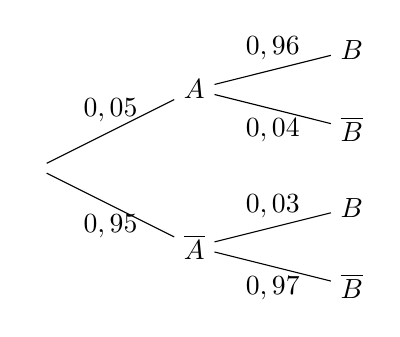
\begin{tikzpicture}[level distance=20mm]  % la longueur des branches
\tikzstyle{level 1}=[sibling distance=20mm] % espace vertical
\tikzstyle{level 2}=[sibling distance=10mm]
\node {} [grow=right]
child {node {$\overline{A}$}
	child {node {$\overline{B}$} 
		edge from parent node[below]{$0,97$}
	}
	child {node {$B$} 
		edge from parent node[above]{$0,03$}
	}
	edge from parent node[below]{$0,95$}
}
child {node {$A$}
	child {node {$\overline{B}$}  
		edge from parent node[below]{$0,04$} 
	}
	child {node {$B$} 
		edge from parent node[above]{$0,96$} 
	}
	edge from parent node[above]{$0,05$}
}; 
\end{tikzpicture}
\end{tcblisting}



\subsection*{Arbre de trois fois deux branches}



\begin{tcblisting}{colback=red!5!white,colframe=red!75!black,listing above text}
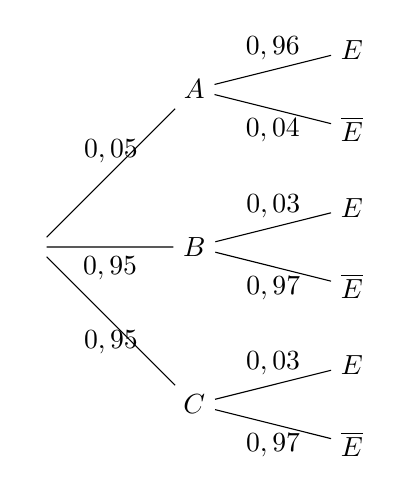
\begin{tikzpicture}[level distance=20mm]
\tikzstyle{level 1}=[sibling distance=20mm]
\tikzstyle{level 2}=[sibling distance=10mm]
\node {} [grow=right]
child {node {$C$}
	child {node {$\overline{E}$} 
		edge from parent node[below]{$0,97$}
	}
	child {node {$E$} 
		edge from parent node[above]{$0,03$}
	}
	edge from parent node[below]{$0,95$}
}
child {node {$B$}
	child {node {$\overline{E}$} 
		edge from parent node[below]{$0,97$}
	}
	child {node {$E$} 
		edge from parent node[above]{$0,03$}
	}
	edge from parent node[below]{$0,95$}
}
child {node {$A$}
	child {node {$\overline{E}$}  
		edge from parent node[below]{$0,04$} 
	}
	child {node {$E$} 
		edge from parent node[above]{$0,96$} 
	}
	edge from parent node[above]{$0,05$}
}; 
\end{tikzpicture}
\end{tcblisting}



\section{Géométrie dans l'espace}


\begin{tcblisting}{colback=red!5!white,colframe=red!75!black,listing above text}
\begin{tikzpicture}[x={(-1cm,-0.3cm)},z={(0cm,1cm)},y={(0.5cm,-0.5cm)}] 
 
\draw[->] (0,0,0)--(5,0,0) node[below] {$x$};
\draw[->] (0,0,0)--(0,5,0) node[right] {$y$};
\draw[->] (0,0,0)--(0,0,5) node[above] {$z$};
\foreach \x in {1,2,3,4} \draw (\x,0,0)--(\x,0.2,0);
\foreach \x in {1,...,5}
	{\draw[color=blue] (0,\x,0)--(0,\x,5);
	\draw[color=blue] (0,0,\x)--(0,5,\x);}
\node[above left] at (1,0,0) {$1$};	
\node[below] at (0,1,0) {$1$};
\node[left] at (0,0,1) {$1$};
\node[below] at (0,0,0) {0};

\draw[dashed] (5,1,4)--(-3,5,0);
\draw[color=green!50!black] plot[mark=*] coordinates {(5,1,4)} node[right]{$A$};
\draw[color=green!50!black] plot[mark=*] coordinates {(3,2,3)} node[right]{$B$};
\draw[color=green!50!black] plot[mark=*] coordinates {(-3,5,0)} node[right]{$C$};

\end{tikzpicture}
\end{tcblisting}
